\chapter{Design und Implementation des Experiments}\label{design}

bla bla bkla kommen wir nun zur implementierung und Entwicklung
hier wichitg aller code steht zur verfügung und kann gerunt werden. Alle benötigten schritte sind in der Arbeit vermekrt (umgebung und so weiter...)


\section{Entwicklungsumgebung}

Um die im folgenden Kapitel \ref{design} beschriebene Implementation lokal durchzuführen, ist es erforderlich, eine geeignete Entwicklungsumgebung aufzusetzen.
Die Programmierung erfolgte mithilfe von Visual Studio Code als Code-Editor. Die Python-Umgebung wurde unter Einsatz des Anaconda Navigators erstellt.
Der gesamte Quellcode basiert auf der Python Version 3.9.16.
Die wichtigsten Bibliotheken für eine erfolgreiche Implementation des nachfolgenden Artefaktes sind Qiskit und PyTorch.
Die Qiskit Version 0.43.0 ist notwendig, da in anderen Versionen von Qiskit Syntaxänderungen auftreten können.

Im Anhang \ref{conda} finden sich eine umfassende Aufstellung aller Abhängigkeiten und Bibliotheken, inklusive ihrer jeweiligen Versionsnummern, die während der Entwicklung und Ausführung des Artefakts zum Einsatz kamen. Zusätzlich sind dort detaillierte Informationen zur Entwicklungsumgebung sowie zur verwendeten Software verfügbar.




\section{Testdatensätze}

Zackige und runde Daten - erzeugt in: dort ausfürhlich dokuemntiert 
aber hier nochmal die websiten: 
Doku bei CODE!

\begin{figure}[htb]
    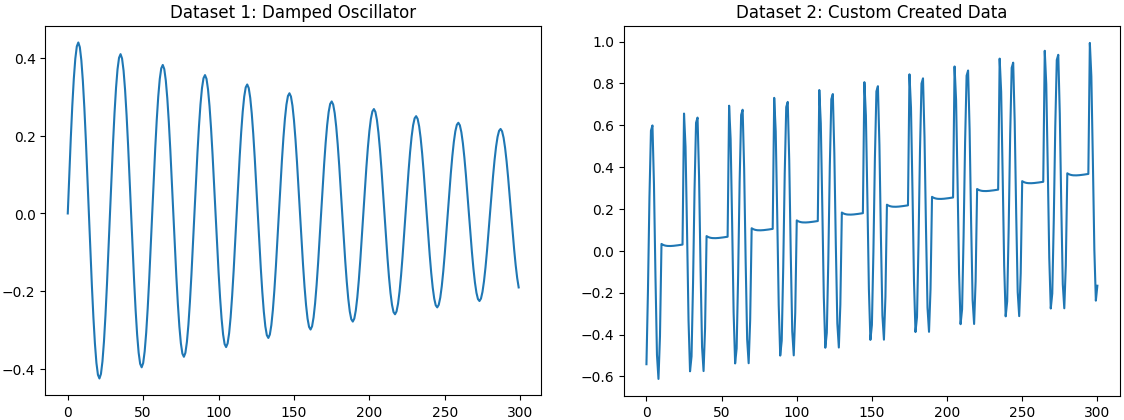
\includegraphics[width=16cm]{lib/graphics/data.png}
    \caption[Testdatensätze]{Testdatensätze}
    \label{abb:datasets}
\end{figure}



\section{Klassische LSTM Architektur Implementation}
als standard

\section{Quantum LSTM Architektur Implementation}
\subsection{Paper 1}
\subsection{Paper 2}

\section{Test Aufbau}

\section{Test Durchführung}
